% Created by tikzDevice version 0.12.3.1 on 2021-08-27 11:08:24
% !TEX encoding = UTF-8 Unicode
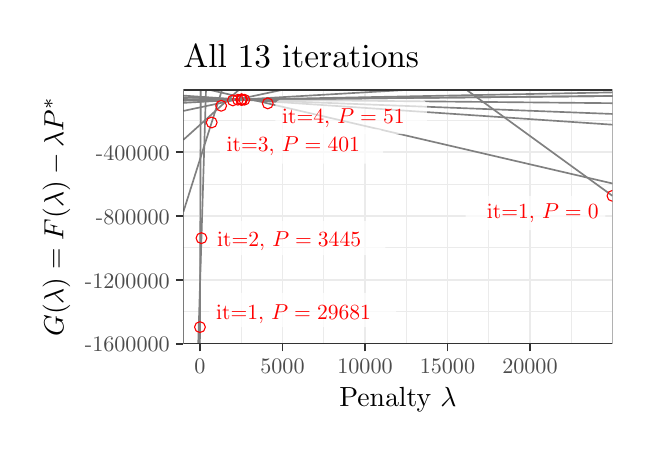
\begin{tikzpicture}[x=1pt,y=1pt]
\definecolor{fillColor}{RGB}{255,255,255}
\path[use as bounding box,fill=fillColor,fill opacity=0.00] (0,0) rectangle (216.81,144.54);
\begin{scope}
\path[clip] (  0.00,  0.00) rectangle (216.81,144.54);
\definecolor{drawColor}{RGB}{255,255,255}
\definecolor{fillColor}{RGB}{255,255,255}

\path[draw=drawColor,line width= 0.6pt,line join=round,line cap=round,fill=fillColor] (  0.00,  0.00) rectangle (216.81,144.54);
\end{scope}
\begin{scope}
\path[clip] ( 56.29, 30.33) rectangle (211.31,122.12);
\definecolor{fillColor}{RGB}{255,255,255}

\path[fill=fillColor] ( 56.29, 30.33) rectangle (211.31,122.12);
\definecolor{drawColor}{gray}{0.92}

\path[draw=drawColor,line width= 0.3pt,line join=round] ( 56.29, 41.87) --
	(211.31, 41.87);

\path[draw=drawColor,line width= 0.3pt,line join=round] ( 56.29, 64.97) --
	(211.31, 64.97);

\path[draw=drawColor,line width= 0.3pt,line join=round] ( 56.29, 88.06) --
	(211.31, 88.06);

\path[draw=drawColor,line width= 0.3pt,line join=round] ( 56.29,111.15) --
	(211.31,111.15);

\path[draw=drawColor,line width= 0.3pt,line join=round] ( 77.16, 30.33) --
	( 77.16,122.12);

\path[draw=drawColor,line width= 0.3pt,line join=round] (106.97, 30.33) --
	(106.97,122.12);

\path[draw=drawColor,line width= 0.3pt,line join=round] (136.78, 30.33) --
	(136.78,122.12);

\path[draw=drawColor,line width= 0.3pt,line join=round] (166.59, 30.33) --
	(166.59,122.12);

\path[draw=drawColor,line width= 0.3pt,line join=round] (196.40, 30.33) --
	(196.40,122.12);

\path[draw=drawColor,line width= 0.3pt,line join=round] (211.31, 30.33) --
	(211.31,122.12);

\path[draw=drawColor,line width= 0.6pt,line join=round] ( 56.29, 30.33) --
	(211.31, 30.33);

\path[draw=drawColor,line width= 0.6pt,line join=round] ( 56.29, 53.42) --
	(211.31, 53.42);

\path[draw=drawColor,line width= 0.6pt,line join=round] ( 56.29, 76.51) --
	(211.31, 76.51);

\path[draw=drawColor,line width= 0.6pt,line join=round] ( 56.29, 99.61) --
	(211.31, 99.61);

\path[draw=drawColor,line width= 0.6pt,line join=round] ( 62.25, 30.33) --
	( 62.25,122.12);

\path[draw=drawColor,line width= 0.6pt,line join=round] ( 92.07, 30.33) --
	( 92.07,122.12);

\path[draw=drawColor,line width= 0.6pt,line join=round] (121.88, 30.33) --
	(121.88,122.12);

\path[draw=drawColor,line width= 0.6pt,line join=round] (151.69, 30.33) --
	(151.69,122.12);

\path[draw=drawColor,line width= 0.6pt,line join=round] (181.50, 30.33) --
	(181.50,122.12);
\definecolor{drawColor}{gray}{0.50}

\path[draw=drawColor,line width= 0.6pt,line join=round] ( 59.10,-867.24) -- ( 65.66,1011.78);

\path[draw=drawColor,line width= 0.6pt,line join=round] ( 56.29,196.34) -- (211.31, 83.77);

\path[draw=drawColor,line width= 0.6pt,line join=round] ( 56.29,-143.74) -- ( 91.70,1011.78);

\path[draw=drawColor,line width= 0.6pt,line join=round] ( 56.29, 78.09) -- (211.31,567.43);

\path[draw=drawColor,line width= 0.6pt,line join=round] ( 56.29,124.26) -- (211.31, 88.24);

\path[draw=drawColor,line width= 0.6pt,line join=round] ( 56.29,104.04) -- (211.31,243.64);

\path[draw=drawColor,line width= 0.6pt,line join=round] ( 56.29,114.46) -- (211.31,147.48);

\path[draw=drawColor,line width= 0.6pt,line join=round] ( 56.29,119.99) -- (211.31,109.48);

\path[draw=drawColor,line width= 0.6pt,line join=round] ( 56.29,117.36) -- (211.31,126.37);

\path[draw=drawColor,line width= 0.6pt,line join=round] ( 56.29,118.14) -- (211.31,121.15);

\path[draw=drawColor,line width= 0.6pt,line join=round] ( 56.29,119.37) -- (211.31,113.36);

\path[draw=drawColor,line width= 0.6pt,line join=round] ( 56.29,118.75) -- (211.31,117.25);

\path[draw=drawColor,line width= 0.6pt,line join=round] ( 56.29,118.35) -- (211.31,119.85);

\path[draw=drawColor,line width= 0.6pt,line join=round] ( 56.29,118.35) -- (211.31,119.85);
\definecolor{fillColor}{RGB}{255,255,255}

\path[fill=fillColor,fill opacity=0.70] ( 67.62, 36.34) --
	(131.16, 36.34) --
	(131.08, 36.34) --
	(131.40, 36.35) --
	(131.71, 36.42) --
	(132.01, 36.53) --
	(132.29, 36.69) --
	(132.54, 36.89) --
	(132.75, 37.13) --
	(132.92, 37.40) --
	(133.05, 37.70) --
	(133.12, 38.01) --
	(133.15, 38.33) --
	(133.15, 38.33) --
	(133.15, 46.71) --
	(133.15, 46.71) --
	(133.12, 47.03) --
	(133.05, 47.34) --
	(132.92, 47.64) --
	(132.75, 47.91) --
	(132.54, 48.15) --
	(132.29, 48.35) --
	(132.01, 48.51) --
	(131.71, 48.62) --
	(131.40, 48.69) --
	(131.16, 48.70) --
	( 67.62, 48.70) --
	( 67.86, 48.69) --
	( 67.54, 48.70) --
	( 67.22, 48.66) --
	( 66.91, 48.57) --
	( 66.62, 48.43) --
	( 66.36, 48.25) --
	( 66.13, 48.03) --
	( 65.94, 47.77) --
	( 65.79, 47.49) --
	( 65.69, 47.19) --
	( 65.64, 46.87) --
	( 65.63, 46.71) --
	( 65.63, 38.33) --
	( 65.64, 38.49) --
	( 65.64, 38.17) --
	( 65.69, 37.85) --
	( 65.79, 37.55) --
	( 65.94, 37.26) --
	( 66.13, 37.01) --
	( 66.36, 36.79) --
	( 66.62, 36.61) --
	( 66.91, 36.47) --
	( 67.22, 36.38) --
	( 67.54, 36.34) --
	cycle;
\end{scope}
\begin{scope}
\path[clip] ( 56.29, 30.33) rectangle (211.31,122.12);
\definecolor{drawColor}{RGB}{255,0,0}

\node[text=drawColor,anchor=base west,inner sep=0pt, outer sep=0pt, scale=  0.78] at ( 68.13, 38.91) {it=1, $P=29681$};
\definecolor{fillColor}{RGB}{255,255,255}

\path[fill=fillColor,fill opacity=0.70] (160.25, 71.41) --
	(206.80, 71.41) --
	(206.72, 71.41) --
	(207.04, 71.42) --
	(207.35, 71.48) --
	(207.65, 71.60) --
	(207.93, 71.76) --
	(208.17, 71.96) --
	(208.39, 72.20) --
	(208.56, 72.47) --
	(208.68, 72.76) --
	(208.76, 73.07) --
	(208.78, 73.39) --
	(208.78, 73.39) --
	(208.78, 81.78) --
	(208.78, 81.78) --
	(208.76, 82.10) --
	(208.68, 82.41) --
	(208.56, 82.70) --
	(208.39, 82.97) --
	(208.17, 83.21) --
	(207.93, 83.41) --
	(207.65, 83.57) --
	(207.35, 83.69) --
	(207.04, 83.75) --
	(206.80, 83.77) --
	(160.25, 83.77) --
	(160.49, 83.75) --
	(160.17, 83.76) --
	(159.85, 83.73) --
	(159.54, 83.64) --
	(159.25, 83.50) --
	(158.99, 83.32) --
	(158.76, 83.10) --
	(158.57, 82.84) --
	(158.42, 82.56) --
	(158.32, 82.25) --
	(158.27, 81.94) --
	(158.26, 81.78) --
	(158.26, 73.39) --
	(158.27, 73.55) --
	(158.27, 73.23) --
	(158.32, 72.92) --
	(158.42, 72.61) --
	(158.57, 72.33) --
	(158.76, 72.08) --
	(158.99, 71.85) --
	(159.25, 71.67) --
	(159.54, 71.54) --
	(159.85, 71.45) --
	(160.17, 71.41) --
	cycle;
\end{scope}
\begin{scope}
\path[clip] ( 56.29, 30.33) rectangle (211.31,122.12);
\definecolor{drawColor}{RGB}{255,0,0}

\node[text=drawColor,anchor=base east,inner sep=0pt, outer sep=0pt, scale=  0.78] at (206.29, 75.46) {it=1, $P=0$};
\definecolor{fillColor}{RGB}{255,255,255}

\path[fill=fillColor,fill opacity=0.70] ( 67.95, 62.31) --
	(127.24, 62.31) --
	(127.16, 62.31) --
	(127.48, 62.32) --
	(127.79, 62.39) --
	(128.09, 62.50) --
	(128.37, 62.66) --
	(128.62, 62.86) --
	(128.83, 63.10) --
	(129.00, 63.37) --
	(129.13, 63.67) --
	(129.20, 63.98) --
	(129.23, 64.29) --
	(129.23, 64.29) --
	(129.23, 72.68) --
	(129.23, 72.68) --
	(129.20, 73.00) --
	(129.13, 73.31) --
	(129.00, 73.60) --
	(128.83, 73.87) --
	(128.62, 74.11) --
	(128.37, 74.32) --
	(128.09, 74.48) --
	(127.79, 74.59) --
	(127.48, 74.65) --
	(127.24, 74.67) --
	( 67.95, 74.67) --
	( 68.19, 74.65) --
	( 67.87, 74.67) --
	( 67.55, 74.63) --
	( 67.24, 74.54) --
	( 66.95, 74.40) --
	( 66.69, 74.22) --
	( 66.46, 74.00) --
	( 66.27, 73.74) --
	( 66.12, 73.46) --
	( 66.02, 73.16) --
	( 65.97, 72.84) --
	( 65.96, 72.68) --
	( 65.96, 64.29) --
	( 65.97, 64.45) --
	( 65.97, 64.13) --
	( 66.02, 63.82) --
	( 66.12, 63.52) --
	( 66.27, 63.23) --
	( 66.46, 62.98) --
	( 66.69, 62.76) --
	( 66.95, 62.57) --
	( 67.24, 62.44) --
	( 67.55, 62.35) --
	( 67.87, 62.31) --
	cycle;
\end{scope}
\begin{scope}
\path[clip] ( 56.29, 30.33) rectangle (211.31,122.12);
\definecolor{drawColor}{RGB}{255,0,0}

\node[text=drawColor,anchor=base west,inner sep=0pt, outer sep=0pt, scale=  0.78] at ( 68.46, 65.62) {it=2, $P=3445$};
\definecolor{fillColor}{RGB}{255,255,255}

\path[fill=fillColor,fill opacity=0.70] ( 71.43, 95.44) --
	(126.47, 95.44) --
	(126.39, 95.45) --
	(126.71, 95.46) --
	(127.02, 95.52) --
	(127.32, 95.64) --
	(127.60, 95.80) --
	(127.85, 96.00) --
	(128.06, 96.24) --
	(128.23, 96.51) --
	(128.36, 96.80) --
	(128.43, 97.11) --
	(128.46, 97.43) --
	(128.46, 97.43) --
	(128.46,105.82) --
	(128.46,105.82) --
	(128.43,106.14) --
	(128.36,106.45) --
	(128.23,106.74) --
	(128.06,107.01) --
	(127.85,107.25) --
	(127.60,107.45) --
	(127.32,107.61) --
	(127.02,107.73) --
	(126.71,107.79) --
	(126.47,107.80) --
	( 71.43,107.80) --
	( 71.67,107.79) --
	( 71.35,107.80) --
	( 71.03,107.76) --
	( 70.72,107.67) --
	( 70.43,107.54) --
	( 70.17,107.36) --
	( 69.94,107.13) --
	( 69.75,106.88) --
	( 69.60,106.60) --
	( 69.50,106.29) --
	( 69.45,105.98) --
	( 69.44,105.82) --
	( 69.44, 97.43) --
	( 69.45, 97.59) --
	( 69.45, 97.27) --
	( 69.50, 96.96) --
	( 69.60, 96.65) --
	( 69.75, 96.37) --
	( 69.94, 96.11) --
	( 70.17, 95.89) --
	( 70.43, 95.71) --
	( 70.72, 95.57) --
	( 71.03, 95.48) --
	( 71.35, 95.45) --
	cycle;
\end{scope}
\begin{scope}
\path[clip] ( 56.29, 30.33) rectangle (211.31,122.12);
\definecolor{drawColor}{RGB}{255,0,0}

\node[text=drawColor,anchor=base west,inner sep=0pt, outer sep=0pt, scale=  0.78] at ( 71.93, 99.79) {it=3, $P=401$};
\definecolor{fillColor}{RGB}{255,255,255}

\path[fill=fillColor,fill opacity=0.70] ( 91.47,106.06) --
	(142.27,106.06) --
	(142.19,106.06) --
	(142.51,106.08) --
	(142.82,106.14) --
	(143.12,106.25) --
	(143.40,106.41) --
	(143.65,106.62) --
	(143.86,106.86) --
	(144.03,107.13) --
	(144.15,107.42) --
	(144.23,107.73) --
	(144.26,108.05) --
	(144.26,108.05) --
	(144.26,116.43) --
	(144.26,116.43) --
	(144.23,116.75) --
	(144.15,117.06) --
	(144.03,117.36) --
	(143.86,117.63) --
	(143.65,117.87) --
	(143.40,118.07) --
	(143.12,118.23) --
	(142.82,118.34) --
	(142.51,118.41) --
	(142.27,118.42) --
	( 91.47,118.42) --
	( 91.71,118.41) --
	( 91.39,118.42) --
	( 91.08,118.38) --
	( 90.77,118.29) --
	( 90.48,118.16) --
	( 90.22,117.97) --
	( 89.99,117.75) --
	( 89.79,117.50) --
	( 89.64,117.21) --
	( 89.54,116.91) --
	( 89.49,116.59) --
	( 89.49,116.43) --
	( 89.49,108.05) --
	( 89.49,108.21) --
	( 89.49,107.89) --
	( 89.54,107.57) --
	( 89.64,107.27) --
	( 89.79,106.99) --
	( 89.99,106.73) --
	( 90.22,106.51) --
	( 90.48,106.33) --
	( 90.77,106.19) --
	( 91.08,106.10) --
	( 91.39,106.06) --
	cycle;
\end{scope}
\begin{scope}
\path[clip] ( 56.29, 30.33) rectangle (211.31,122.12);
\definecolor{drawColor}{RGB}{255,0,0}

\node[text=drawColor,anchor=base west,inner sep=0pt, outer sep=0pt, scale=  0.78] at ( 91.98,109.97) {it=4, $P=51$};

\path[draw=drawColor,line width= 0.4pt,line join=round,line cap=round] ( 62.25, 36.34) circle (  1.96);

\path[draw=drawColor,line width= 0.4pt,line join=round,line cap=round] (211.31, 83.77) circle (  1.96);

\path[draw=drawColor,line width= 0.4pt,line join=round,line cap=round] ( 62.80, 68.49) circle (  1.96);

\path[draw=drawColor,line width= 0.4pt,line join=round,line cap=round] ( 66.49,110.28) circle (  1.96);

\path[draw=drawColor,line width= 0.4pt,line join=round,line cap=round] ( 86.75,117.19) circle (  1.96);

\path[draw=drawColor,line width= 0.4pt,line join=round,line cap=round] ( 69.92,116.31) circle (  1.96);

\path[draw=drawColor,line width= 0.4pt,line join=round,line cap=round] ( 74.14,118.26) circle (  1.96);

\path[draw=drawColor,line width= 0.4pt,line join=round,line cap=round] ( 78.30,118.50) circle (  1.96);

\path[draw=drawColor,line width= 0.4pt,line join=round,line cap=round] ( 75.98,118.51) circle (  1.96);

\path[draw=drawColor,line width= 0.4pt,line join=round,line cap=round] ( 77.15,118.55) circle (  1.96);

\path[draw=drawColor,line width= 0.4pt,line join=round,line cap=round] ( 77.45,118.55) circle (  1.96);

\path[draw=drawColor,line width= 0.4pt,line join=round,line cap=round] ( 77.33,118.55) circle (  1.96);

\path[draw=drawColor,line width= 0.4pt,line join=round,line cap=round] ( 77.28,118.55) circle (  1.96);

\path[draw=drawColor,line width= 0.4pt,line join=round,line cap=round] ( 77.29,118.55) circle (  1.96);
\definecolor{drawColor}{gray}{0.20}

\path[draw=drawColor,line width= 0.6pt,line join=round,line cap=round] ( 56.29, 30.33) rectangle (211.31,122.12);
\end{scope}
\begin{scope}
\path[clip] (  0.00,  0.00) rectangle (216.81,144.54);
\definecolor{drawColor}{gray}{0.30}

\node[text=drawColor,anchor=base east,inner sep=0pt, outer sep=0pt, scale=  0.80] at ( 51.34, 27.37) {-1600000};

\node[text=drawColor,anchor=base east,inner sep=0pt, outer sep=0pt, scale=  0.80] at ( 51.34, 50.46) {-1200000};

\node[text=drawColor,anchor=base east,inner sep=0pt, outer sep=0pt, scale=  0.80] at ( 51.34, 73.56) {-800000};

\node[text=drawColor,anchor=base east,inner sep=0pt, outer sep=0pt, scale=  0.80] at ( 51.34, 96.65) {-400000};
\end{scope}
\begin{scope}
\path[clip] (  0.00,  0.00) rectangle (216.81,144.54);
\definecolor{drawColor}{gray}{0.20}

\path[draw=drawColor,line width= 0.6pt,line join=round] ( 53.54, 30.33) --
	( 56.29, 30.33);

\path[draw=drawColor,line width= 0.6pt,line join=round] ( 53.54, 53.42) --
	( 56.29, 53.42);

\path[draw=drawColor,line width= 0.6pt,line join=round] ( 53.54, 76.51) --
	( 56.29, 76.51);

\path[draw=drawColor,line width= 0.6pt,line join=round] ( 53.54, 99.61) --
	( 56.29, 99.61);
\end{scope}
\begin{scope}
\path[clip] (  0.00,  0.00) rectangle (216.81,144.54);
\definecolor{drawColor}{gray}{0.20}

\path[draw=drawColor,line width= 0.6pt,line join=round] ( 62.25, 27.58) --
	( 62.25, 30.33);

\path[draw=drawColor,line width= 0.6pt,line join=round] ( 92.07, 27.58) --
	( 92.07, 30.33);

\path[draw=drawColor,line width= 0.6pt,line join=round] (121.88, 27.58) --
	(121.88, 30.33);

\path[draw=drawColor,line width= 0.6pt,line join=round] (151.69, 27.58) --
	(151.69, 30.33);

\path[draw=drawColor,line width= 0.6pt,line join=round] (181.50, 27.58) --
	(181.50, 30.33);
\end{scope}
\begin{scope}
\path[clip] (  0.00,  0.00) rectangle (216.81,144.54);
\definecolor{drawColor}{gray}{0.30}

\node[text=drawColor,anchor=base,inner sep=0pt, outer sep=0pt, scale=  0.80] at ( 62.25, 19.46) {0};

\node[text=drawColor,anchor=base,inner sep=0pt, outer sep=0pt, scale=  0.80] at ( 92.07, 19.46) {5000};

\node[text=drawColor,anchor=base,inner sep=0pt, outer sep=0pt, scale=  0.80] at (121.88, 19.46) {10000};

\node[text=drawColor,anchor=base,inner sep=0pt, outer sep=0pt, scale=  0.80] at (151.69, 19.46) {15000};

\node[text=drawColor,anchor=base,inner sep=0pt, outer sep=0pt, scale=  0.80] at (181.50, 19.46) {20000};
\end{scope}
\begin{scope}
\path[clip] (  0.00,  0.00) rectangle (216.81,144.54);
\definecolor{drawColor}{RGB}{0,0,0}

\node[text=drawColor,anchor=base,inner sep=0pt, outer sep=0pt, scale=  1.00] at (133.80,  7.62) {Penalty $\lambda$};
\end{scope}
\begin{scope}
\path[clip] (  0.00,  0.00) rectangle (216.81,144.54);
\definecolor{drawColor}{RGB}{0,0,0}

\node[text=drawColor,rotate= 90.00,anchor=base,inner sep=0pt, outer sep=0pt, scale=  1.00] at ( 12.89, 76.22) {$G(\lambda)=F(\lambda)-\lambda P^*$};
\end{scope}
\begin{scope}
\path[clip] (  0.00,  0.00) rectangle (216.81,144.54);
\definecolor{drawColor}{RGB}{0,0,0}

\node[text=drawColor,anchor=base west,inner sep=0pt, outer sep=0pt, scale=  1.20] at ( 56.29,130.17) {All 13 iterations};
\end{scope}
\end{tikzpicture}
